%
% File emnlp2018.tex
%
%% Based on the style files for EMNLP 2018, which were
%% Based on the style files for ACL 2018, which were
%% Based on the style files for ACL-2015, with some improvements
%%  taken from the NAACL-2016 style
%% Based on the style files for ACL-2014, which were, in turn,
%% based on ACL-2013, ACL-2012, ACL-2011, ACL-2010, ACL-IJCNLP-2009,
%% EACL-2009, IJCNLP-2008...
%% Based on the style files for EACL 2006 by 
%%e.agirre@ehu.es or Sergi.Balari@uab.es
%% and that of ACL 08 by Joakim Nivre and Noah Smith

\documentclass[11pt,a4paper]{article}
\usepackage[hyperref]{emnlp2018}
\usepackage{times}
\usepackage{latexsym}
\usepackage{graphicx, amsmath, verbatim}

%\usepackage{url}

% \aclfinalcopy % Uncomment this line for the final submission

%\setlength\titlebox{5cm}
% You can expand the titlebox if you need extra space
% to show all the authors. Please do not make the titlebox
% smaller than 5cm (the original size); we will check this
% in the camera-ready version and ask you to change it back.

\newcommand\BibTeX{B{\sc ib}\TeX}
\newcommand\confname{EMNLP 2018}
\newcommand\conforg{SIGDAT}

\title{Instructions for \confname{} Proceedings}

\author{First Author \\
  Affiliation / Address line 1 \\
  Affiliation / Address line 2 \\
  Affiliation / Address line 3 \\
  {\tt email@domain} \\}

\date{}

\begin{document}
\maketitle
\begin{abstract}
  This document contains the instructions for preparing a camera-ready
  manuscript for the proceedings of \confname{}. The document itself
  conforms to its own specifications, and is therefore an example of
  what your manuscript should look like. These instructions should be
  used for both papers submitted for review and for final versions of
  accepted papers.  Authors are asked to conform to all the directions
  reported in this document.
\end{abstract}

\section{Introduction}
Sentiment analysis is a multifaceted task, involving the identification and classification of opinion expressions, the identification of opinion holders, and the identification of opinion targets.
% characterize the polarity of that opinion and the strength of that opinion.
Historically, research in sentiment analysis has focused on finding the overall sentiment of a short span of text, like tweets (), product reviews () or movie reviews ().
However, in recent years, there has been a shift towards more fine-grained opinion mining.
Not only is the overall sentiment of a piece of text to be determined, but the opinion holder and target are also identified, allowing for a much more nuanced understanding of the sentiments expressed within a text.
\par With few exceptions, much of the work in fine-grained sentiment analysis () has focused on classifying sentiments within a single sentence, containing a single entity pair mention.
However, sentiments are expressed in all types of texts, many of which are contain multiple sentences, multiple entity pairs, and multiple mentions of each entity.
News articles in particular often encode complex networks of opinions amongst a multitude of entities.
Take this article from Xinhua News Agency as an example, where various types of sentiments are expressed amongst the seven different entities identified in the article:
\begin{figure} \label{fig:intro}
\centering
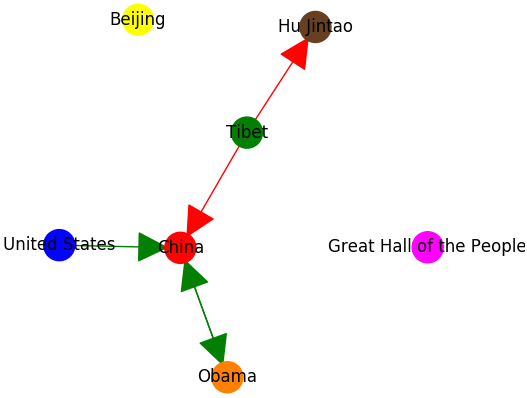
\includegraphics[scale=0.5]{example_article.png}
\caption{Graph showing the network of sentiments expressed amongst various entities in the example article. Arrows are directed from opinion holder to opinion target. \textcolor{red}{Red} arrows indicate negative sentiment and \textcolor[rgb]{0, 0.5, 0}{green} arrows indicate positive sentiment. Disconnected nodes represent entities that are present in the text, but do not participate in any sentiment relations, either as opinion holders or opinion targets.}
\end{figure}
\begin{quote}
URGENT: \textcolor[rgb]{1, 0.5, 0}{\textbf{Obama}} says \textcolor[rgb]{0, 0, 1}{\textbf{U.S.}} recognizes \textcolor[rgb]{0, 0.5, 0}{\textbf{\textcolor[rgb]{0, 0.5, 0}{\textbf{Tibet}} as part of \textcolor[rgb]{1, 0, 0}{\textbf{China}}}}. \textcolor[rgb]{0, 0, 1}{\textbf{United States}} President \textcolor[rgb]{1, 0.5, 0}{\textbf{Barack Obama}} Tuesday said the \textcolor[rgb]{0, 0, 1}{\textbf{U.S.}} government recognizes that \textcolor[rgb]{0, 0.5, 0}{\textbf{Tibet}} is \textcolor[rgb]{0, 0.5, 0}{\textbf{part of the \textcolor[rgb]{1, 0, 0}{\textbf{People's Republic of China}}}}. He also said that \textcolor[rgb]{0, 0, 1}{\textbf{the \textcolor[rgb]{0, 0, 1}{\textbf{United States}}}} supports the early resumption of dialogue between the \textcolor[rgb]{1, 0, 0}{\textbf{Chinese}} government and representatives of the Dalai Lama to resolve any concerns and differences that the two sides may have. ``\textcolor[rgb]{0, 0, 1}{\textbf{The \textcolor[rgb]{0, 0, 1}{\textbf{United States}}}} respects the sovereignty and territorial integrity of \textcolor[rgb]{1, 0, 0}{\textbf{China}},'' \textcolor[rgb]{1, 0.5, 0}{\textbf{Obama}} said at a joint press conference with \textcolor[rgb]{1, 0, 0}{\textbf{Chinese}} President \textcolor[rgb]{0.4, 0.25, 0.13}{\textbf{Hu Jintao}} at \textcolor[rgb]{1, 1, 0}{\textbf{Beijing}}'s \textcolor[rgb]{1, 0, 1}{\textbf{Great Hall of the People}}.
\end{quote}
Five sentiments have been labelled within this article:
\begin{enumerate}
\item \textcolor[rgb]{1, 0.5, 0}{\textbf{Obama}} is \textcolor[rgb]{0, 0.5, 0}{positive} towards \textcolor[rgb]{1, 0, 0}{\textbf{China}}
\item \textcolor[rgb]{0, 0, 1}{\textbf{United States}} is \textcolor[rgb]{0, 0.5, 0}{positive} towards \textcolor[rgb]{1, 0, 0}{\textbf{China}}
\item \textcolor[rgb]{1, 0, 0}{\textbf{China}} is \textcolor[rgb]{0, 0.5, 0}{positive} towards \textcolor[rgb]{1, 0.5, 0}{\textbf{Obama}}
\item \textcolor[rgb]{0, 0.5, 0}{\textbf{Tibet}} is \textcolor[rgb]{1, 0, 0}{negative} towards \textcolor[rgb]{1, 0, 0}{\textbf{China}}
\item \textcolor[rgb]{0, 0.5, 0}{\textbf{Tibet}} is \textcolor[rgb]{1, 0, 0}{negative} towards \textcolor[rgb]{0.4, 0.25, 0.13}{\textbf{Hu Jintao}}
\end{enumerate}
The fifth sentiment, in particular, involves entities that are never even mentioned in the same sentence, and thus cannot be extracted by sentence-level models.
\par To create complex sentiment networks for articles, we formulate the task in a pipelined manner.
In the first step, all entities within a document are extracted and labelled.
Co-reference resolution is performed to identify all mentions of each entity.
In the second step, we consider each pair of entities and classify their sentiment relationship into three possible types: positive, negative, or none.
This is opposed to previous approaches which first identified sentiment of a text, and then the holder and target of that sentiment ().
Such an approach works well for short texts like reviews, which express a single main sentiment between a single holder-target pair, but works less well for long documents in which multiple entities participate in various sentiment relations.
As strong NER () and coreference~\cite{Lee:17} models exist already, we focus the bulk of our work on the second task, allocating the first task to preprocessing.
We propose a novel neural architecture for this task, and show that it outperforms sentence-level baselines.
% (discuss more formulation later, just touch upon here)

\section{Data}

% Data statistics
\begin{table*}[!t]
\centering
\begin{tabular}{| l | r | r | r | r | r | r |}
\hline
 & & Entities & & & & \\
Dataset & Docs & / Doc & Neg & None & Pos & \% None \\ \hline \hline
train-original & 897 & 2.63 & 648 & 815 & 355 & 44.8 \\
train-new & 949	 & 8.98 & 973 & 11306 & 1013 & 85.1 \\
dev-tune & 38 & 8.82 & 158 & 2349 & 365 & 81.8 \\
dev-eval& 37 & 9.08 & 174 & 2454 & 404 & 80.9 \\
test-KBP & 79 & 9.25 & 437 & 5459 & 718 & 82.5 \\
test-MPQA & 54 & 11.72 & 521 & 6464 & 625 & 84.9 \\
\hline
\end{tabular}
\caption{\label{tab:data} Dataset statistics. For each dataset, shows the total number of articles, the average number of entities within each article, the total number of negative pairs, none pairs, positive pairs, and the percentage of all pairs that are none.}
\end{table*}

We use datasets from~\shortcite{Choi:16} for training, development, and testing.
~\shortcite{Choi:16} introduces five datasets for document-level sentiment extraction, each containing a collection short documents that are densely annotated at the entity-level, but not the mention-level.
The training set (``train-original") comprises of news articles from the Gigaword corpus ().
Human-annotated labels were generated for this set via crowdsourcing.
Two separate development sets, one for hyper-parameter tuning (``dev-tune") and one for evaluation (``dev-eval"), were also introduced, split off from the existing KBP dataset.
As the KBP set had been sparsely-labelled, the gold-standard annotations for this set were supplemented with human annotations to create labels between all entity pairs.
The KBP set was then split, with 50\% of the documents being used for development: 25\% for tuning and 25\% for 
evaluation. The other 50\% was reserved for testing (``test-KBP").
A second test set (``test-MPQA") was also used, derived from densely-labelled MPQA dataset.
The four development and test datasets have labels for all entities pair within its documents.

\subsection{Training Data}
\par The distribution of the original training set does not mimic that of the development and test sets, most notably due to its lack of ``none" labels.
Such domain differences can problematic for deep neural networks in NLP~\cite{Mou:16}.
Therefore, to optimize our model's performance, we make two changes to the training set.
First, we incorporate dev-tune into our training set, using dev-eval for both hyper-parameter tuning and evaluation.
As dev-tune, dev-eval, and test-KBP are all derived from the same corpus, their distributions should match.
Second, we supplement the training data with weakly generated ``none" pairs.
As the original training set did not have annotations between all pairs of entities within a document, we can generate new examples by finding un-labelled pairs and assuming those pairs hold no sentiment.
We randomly select 10\% of the newly generated pairs and add them to the training data, which was sufficient to increase the proportion of ``none" pairs in the training data to 85\%, comparable to the 80-85\% found in the development and test sets. % cite table here?
Table \ref{tab:data} shows that the distribution of the new training dataset (``train-new") is now much closer to that of the development and test sets.
% The statistics for the old and new training data, as well as the development and test data, are fond in table \ref{tab:data}

\subsection{Preprocessing}
We use preprocessed data from~\shortcite{Choi:16}, discarding part-of-speech tags and dependency paths which are not used by our model.
Instead, the preprocessing pipeline for our model consists of only three steps: tokenization, NER, and co-reference resolution.
Stanford CoreNLP~\cite{Manning:14} was used for all three steps.
Following NER, entities of type date, duration, money, time, and number were discarded, as they do not tend to participate in sentiment relations.
Coreference resolution was performed on the remaining entities to isolate all mentions of the entity
Several heuristics were applied to identify named entities which refer to the same entity, and all mentions of those entities were merged into a single co-reference chain.

\section{Models}
We formulate our task by considering all entities within a document as potential holders and targets of sentiments. If there are $E$ entities in the document, then we consider $E(E - 1)$ holder-target pairs for the document.
For each pair, we classify its sentiment into one of $\{$positive$,$ negative$,$ none$\}$.
% whether a sentiment exists from the holder to the target, and whether the sentiment is positive or negative.
We explore two different neural models for this task.

\subsection{Multi-layer BiLSTM}
\noindent\textbf{Inputs.}
We concatenate three sets of embeddings to represent each token $x_t$: word embeddings ($w_t$), learned polarity embeddings ($p_t$), and learned holder-target embeddings ($e_t$):
	$$x_t = [w_t, p_t, e_t]$$
Pre-trained GloVe vectors~\cite{Pennington:14} are used for word embeddings.
We also explicitly encode the polarity of known subjectivity clues by appending embeddings for its polarity.
Subjectivity clues refer to words which may be used subjectively, in either a positive or negative context.
We use a pre-existing lexicon of over 8000 subjectivity clues from~\shortcite{Wilson:05} and learn different embeddings for strongly positive, weakly positive, strongly negative, weakly negative, and neutral words.
Finally, as our model architecture has no notion of which words are holders and which are targets, we rely on a holder-target embedding to encode whether each token is part of a holder span, part of a target span, or not part of either.

\noindent\textbf{LSTM.}
We feed each embedded token $x_t$ into a bidirectional LSTM to encode it within its context.
\begin{align*}
f_{t, \delta} & = \sigma(\textbf{W}_f [x_t, h_{t + \delta, \delta}] + b_i) \\
o_{t, \delta} & = \sigma(\textbf{W}_o[x_t, h_{t + \delta,\delta}] + b_o) \\
\tilde{c}_{t, \delta} & = \tanh(\textbf{W}_c[x_t, h_{t + \delta, \delta}] + b_c) \\
c_{t, \delta} & = f_{t, \delta}\circ \tilde{c}_{t, \delta} + (1 - f_{t, \delta})\circ c_{t + \delta, \delta} \\
h_{t, \delta} & = o_{t, \delta}\circ \tanh(c_{t,\delta}) \\
x^*_t & = [h_{t, 1}, h_{t, -1}]
\end{align*}
whereby $\delta = \{1, -1\}$ indicates directionality of the LSTM.
The final representation of the token $x_t^*$ is a concatenation of the output from the forward LSTM and that from the backward LSTM.

\noindent\textbf{Attention.}
We use an attentional mechanism over all contextually-encoded tokens $x_t^*\in \{x_0^*, \dots, x_T^*\}$ to extract a final sentiment score $s_{i, j}$ from holder $i$ to target $j$.
\begin{align*}
\alpha_{t} & = \textbf{W} \cdot x^*_t \\
a_{i, j, t} & = \frac{\exp{(\alpha_t)}}{\sum^{T}_{k=0} \exp{(\alpha_k)}} \\
s_{i, j} & = \sum^{T}_{t = 0} a_{i, j, t}\cdot x_t^*
\end{align*}

\noindent\textbf{Hyperparameters.}
The GloVe embeddings, learned polarity embeddings, and learned holder-target embeddings are 50-dimensional each.
For the biLSTM, we use 2 stacked layers and a hidden dimension of 50. We apply a dropout to the hidden layer of the LSTM with probability 0.2.
For training, we optimize the model using Adam with $\alpha$ = 1e-3, $\beta_1$ = 0.9, $\beta_2$ = 0.999, $\epsilon$ = 1e-8. We use a batch size of 50, training up to 15 epochs, with epoch 6 being selected as the optimal epoch based on development set performance.

\subsection{Advanced Model} % rename this
We introduce a novel architecture for the classification of opinion sentiment.
This model is built off of the multi-layer biLSTM, with additional connections added on top to encapsulate the holder-target relationship.
We also borrow components of this model from state-of-the-art models in relation extraction~\cite{Verga:18} and co-reference resolution~\cite{Lee:17}.

\noindent\textbf{Inputs.}
We concatenate two sets of embeddings to represent each token $x_t$: word embeddings ($w_t$) and polarity embeddings ($p_t$):
	$$x_t = [w_t, p_t]$$
Both embeddings are identically set up to those used in the multi-layer biLSTM.
Note that we do not need to append holder-target embeddings as the relation is built into the model architecture itself.

\noindent\textbf{LSTM.}
We use the LSTM component of the multi-layer biLSTM to contextually encode each embedded token $x_t$.
	$$x^*_t = [h_{t, 1}, h_{t, -1}]$$
Once again, the final representation $x^*_t$ is a concatenation of the output from the forward LSTM and that from the backward LSTM.

\noindent\textbf{Span Representations.}
To represent multi-word mentions and entities (``spans"), we use span representations based on those used by~\shortcite{Lee:17}.
For each span $i$, we take the LSTM-encoded tokens in the span and concatenate them in the following manner:
\begin{equation*}
\textbf{g}_i = [x^*_{START(i)}, x^*_{END(i)}, \hat{\textbf{x}}_i]
\end{equation*}
whereby $\textbf{x}^*_{START(i)}$ and $\textbf{x}^*_{END(i)}$ are the endpoints of the span, and $\hat{\textbf{x}}_t$ is computed using an attention mechanism over each embedded word in the span.
%The attention weights $a_{i,t}$ are computed using a feed-forward network, and normalized with softmax.
Following \cite{Lee:17}'s work, we compute the attentive representation $\hat{\textbf{x}}_i$ is computed as a weighted sum of each embedded word $x_t$ in the span.
We make a slight modification in that we compute attention directly from the embedded token themselves, rather than deriving them from the LSTM-encoded outputs.
\begin{align*}
	\alpha_t & = \textbf{w}_\alpha \cdot FFNN_\alpha (x_t) \\
	a_{i, t} & = \frac{\exp{(\alpha_t)}}{\sum^{END(i)}_{k=START(i)} \exp{(\alpha_k)}} \\
	\hat{\textbf{x}}_i & = \sum^{END(i)}_{t = START(i)} a_{i, t}\cdot x_t
\end{align*}

\noindent\textbf{Pairwise Scoring.}
~\shortcite{Verga:18} scores pairs of triples using an MLP followed by a bilinear operator.
To minimize the number of parameters, we instead use a linear transformation of concatenated holder-target representations. 
We represent all pairs of the $n$ holder mentions $\textbf{g}_{1}^{holder}, \textbf{g}_{2}^{holder},\dots,\textbf{g}_{n}^{holder}$ and the $m$ target mentions $\textbf{g}_{1}^{target}, \textbf{g}_{2}^{target},\dots,\textbf{g}_{m}^{target}$ using concatenation, generating a total of $n\cdot m$ pair representations.
	$$\textbf{p}_{i, j} = [\textbf{g}_i^{holder}, \textbf{g}_j^{target}, \phi(i, j)]$$
where $\phi$ represents feature vectors for the pair $(i, j)$.
We then apply a linear mapping to generate scores for all mention pairs, for each of the 3 possible sentiments. We generate separate scores for each (holder mention $i$, target mention $j$, sentiment $s$) triple, where $s\in\{$positive, negative, none$\}$.
	$$A_{i, j, s} = \textbf{M}\cdot \textbf{p}_{i,j}$$

% present "failure" in right way
% discuss everything that was tried

\noindent\textbf{Features.}
For each holder-target mention pair, we learn separate embeddings for four different sets of features,
	$$\phi(i, j) = [\phi_s(i, j),  \phi_c(i, j), \phi_f(i, j), \phi_r(i, j)]$$
which, as noted above, we append to its pairwise representation.
$\phi_s$ encodes how the sentence baseline predicted the example, with different embeddings for positive, negative, and no sentiment predictions.
$\phi_c$ is a co-occurrence feature, representing the number of sentences in which the holder and target both appeared.
Finally, we have features $\phi_f$ and $\phi_r$ encoding the total number of mentions of the holder entity and target entity.
Whereas $\phi_f$ (``frequency") encodes the raw number of mentions of each entity, $\phi_r$ (``rank") encodes the ``rank" of the entity, with the most frequently mentioned entity ranked 1, the second-most frequently mentioned ranked 2, and so on.
Importantly, note all these features remain constant for all mentions of the same entity pair.

\noindent\textbf{Aggregation.}
Our data contains labels for each entity pair, but not for each mention pair.
To deal with this, we perform multi-instance learning following~\shortcite{Verga:18}, whereby we train the model over the aggregate of the mention pairs and perform a single update for the aggregate.
We use LogSumExp as the aggregation function. The LogSumExp function is a smooth approximation of the max, allowing us to extract the most probable scores for each sentiment $s$.
\begin{align*}
	score(\text{holder}, & \text{ target}, s) \\
	& = \log\sum_{\substack{i\in \{1,\dots n\},\\ j\in \{1,\dots m\}}}\exp{(A_{i, j, s})}
\end{align*}

\noindent\textbf{Training.}
We aim to maximize the log-likelihood of the correct labels for each example.
We can represent each example by the triple $(\text{document }D, \text{ holder entity }h, \text{ target entity }t)$.
\par Let $\mathcal{Y} = \{\text{Positive}, \text{ Negative}, \text{ None}\}$ represent the set of all possible labels for each example.
Given $N$ training examples labelled $y_1,\dots, y_n\in \mathcal{Y}$, with document $D$, the likelihood is given by
\begin{align*}
	P(y_1, & \dots, y_n | D, h, t) \\
	& = \prod_{i=1}^N P(y_i | D, h, t) \\
	& = \prod_{i=1}^N \frac{\exp{(score(h, t, y_i))}}{\sum_{y'\in \mathcal{Y}} \exp{(score(h, t, y'))}}
\end{align*}
We aim to maximize the the log-likelihood
	$$\sum_{i=1}^N \log{\Big(\frac{\exp{(score(h, t, y_i))}}{\sum_{y'\in \mathcal{Y}} \exp{(score(h, t, y'))}}\Big)}$$
% Probabilities here 

\noindent\textbf{Hyperparameters.}
The GloVe embeddings and learned polarity embeddings are 50-dimensional each.
All features are represent as 25-dimensional learned embeddings. The co-occurrence feature $\phi_c$ are binned into buckets: [0, 1, 2, 3, 4, 5, 6, 7, 8, 9, 10+]. The mention features $\phi_f$ and $\phi_r$ are binned into [1, 2, 3, 4, 5+].
For the biLSTM, we use 2 stacked layers and a hidden dimension of 50. We apply a dropout to the input and all hidden layers of the LSTM with probability 0.2.
For training, we optimize the model using Adam with $\alpha$ = 1e-3 and a weight decay of 1e-5. We also set $\beta_1$ = 0.9, $\beta_2$ = 0.999, $\epsilon$ = 1e-8. We use a batch size of 50 and train up to 10 epochs, with epoch 6 being selected as the optimal epoch based on development set performance.

\section{Results}
We use F1 scores as the metric for model performance on this task.
We report the precision, recall, and F1 scores of each sentiment class in table \ref{tab:results}.
In general, our model, which has the capacity to perform cross-sentence reasoning, performs significantly better than sentence-level baselines.
For all neural models, recall is much higher than precision if there is a sentiment, while precision is much higher than recall if there is no sentiment. Notably, while our F1 scores on positive and negative sentiment do not exceed that of~\shortcite{Choi:16}, our recalls are much higher than theirs. This suggests that neural models tend to more conservative in picking ``no sentiment" labels. This additionally suggests that combining aspects of both models may be beneficial.

\subsection{Sentence Baseline}
~\shortcite{Socher:13} introduced a sentence-level RNN model for classifying the sentiment of sentences.
The model takes a sentence as input and classifies its sentiment into five possible classes: very negative, negative, neutral, positive, and very positive.
We use an adaptation of this model to encapsulate how sentence-level models will perform on our task.
To classify a holder-target pair, we begin by collecting all sentences in which the holder and target entities co-occur.
We then classify each of the sentences according to ~\shortcite{Socher:13}'s model.
We classify the pair's sentiment as `none' if the entities do not co-occur in any sentence or if all sentences in which the entities co-occur in are classified as `neutral.'
We classify the pair's sentiment as `positive' if at least one sentence in which the entities co-occur in is classified as `positive' or 'very positive.'
Otherwise, we classify the pair's sentiment as `negative.' % (if at least one sentence in which the entities co-occur is classified as `negative' or 'very negative', and no sentences are classified as `positive.')
Domain differences are the motivation for this split proportion, specifically the fact that positive labels can be up to two times more frequent than negative labels in our dataset.
\par Note that such a model assumes that any sentence in which holder and target entities co-occur express a single sentiment, and that the sentiment expressed in the sentence is the sentiment between the entity pair.
% However, these assumptions are not unreasonable, and most sentence-level approaches to fine-grained sentiment analysis also make these assumptions.
Both assumptions represent implicit limitations in sentence-level models.
Current pipelined approaches to sentence-level fine-grained sentiment analysis, which first isolate sentiments before isolating the holders and targets of that sentiment (), also make these assumptions.
Moreover, sentence-level models assume that entities which aren't mentioned in the same sentence do not express a sentiment, which again their inhibits performance on document-level tasks.

\subsection{SVM and SVM+ILP Baseline}
As additional baselines for comparison, we report positive and negative F1 scores from~\shortcite{Choi:16}, which is state-of-the-art for document-level entity-entity sentiment extraction.
In~\shortcite{Choi:16}'s SVM+ILP model, social science theories were encoded as soft ILP constraints on top of a base SVM pairwise classifier.
We report results from both the SVM base classifier and the SVM+ILP classifier with encoded constraints.
While our model does not ultimately outperform the final SVM+ILP classifier, it comes to within 2-3 points of the SVM base classifier.
It also has significantly higher recall than either classifier.

% Add table here

\subsection{Ablations}
Results from ablating our model are shown in table ~\ref{tab:ablations}.
We report performance on the development data for our ablation study.
In particular, we focus on the effect of removing features.
Features for number of mentions ($\phi_f$ and $\phi_r$) contribute the most to the final results, perhaps due to how predictive they are for whether entity pairs do or do not hold sentiment.
% Analysis shows that _ % of scores were positive, _ % were negative
Discerning whether or not sentiment was present was by far the most challenging task for the model, thus explaining why our model would benefit from such feature.
% ^Verify this
Co-occurrence features ($\phi_c$) are the next largest contributors to the final results.

\subsection{Error Analysis of Neural Models}
% All error analysis done on dev data
\noindent\textbf{Sentence Baseline}
% Does it actually learn cross-sentence relations? (vs. something like the sentence baseline)
% how much of the errors of the sentence baseline is due to mislabelling of sentence vs. how much is due to entities which co-occur has sentence not vs. how much is due to failing to account for cross-sentence entities (i.e. mislabelling entities which do not co-occur in the same sentence) vs. how much is due to assuming sentiment of sentences entities encapsulates sentiment between entities
% now repeat for the advanced model
% The most major source of error in the sentence baseline: sentence's sentiment does not align with actual sentiment between entities
% Moreover, of the entities that co-occurred once, 73% of them do not hold sentiment. However, only 4% of the sentences they co-occur are neutral in sentiment. This heavily implying that, in practice for longer documents, most sentences in which two entities co-occur in do not encapsulate the sentiment between the entities, marking a limitation of sentence-level models.
% These examples, in which the sentiment of the sentence the entities co-occur in do not match the actual sentiment between entities accounts for at least 73% of all errors (Footnote: even this number is an underestimate; we say "at least" because only count for entities which co-occurred once in computing this figure. These entities account for 82% of all co-occurring entities, however, so the number should be fairly accurate)

% Second largest source of error from always classifying non-co-occurring pairs as "none."
In our data, at least 22\% of negatively-labelled pairs and 28\% of positively-labelled pairs do not co-occur in a sentence.
% Sentence baseline classifies all of these as none, counting for 153 of errors (14% of errors)
% Sentence baseline makes a total of 1100 errors

\noindent\textbf{Multi-layer BiLSTM and Advanced Model} % Rename this
% As noted in sentence baseline, large issue: 
% Advanced model does learn to classify pairs that do not co-occur in a sentence as 
% In fact advanced model is over-zealous in doing so, and 39% of its predicted negative pairs and 35% of its predicted positive pairs do not co-occur in any sentence
% Of the 153 pairs, how many are classified correctly?
Both the biLSTM and the advanced model are overzealous in classifying non-co-occurring pairs as holding sentiment. % However, this may just be because of general trend of classifying no sentiment pairs as having sentiment

Surprisingly, the vanilla version of the (advanced model) without any features does not outperform the multi-layer biLSTM.
However, with the addition of features, this model receives a boost in performance, significantly outperforming the multi-layer biLSTM.


\subsection{Error Analysis}
% Predisposition to add extra labels.
\noindent\textbf{Sentiment vs. No Sentiment.}
% Table showing breakdown of labels & how they were predicted. By far largest mistake is no sentiment/sentiment

\section{Related Work}

\section{Conclusion}

\section*{Acknowledgments}
The acknowledgments should go immediately before the references.  Do
not number the acknowledgments section. Do not include this section
when submitting your paper for review. \\

\noindent {\bf Preparing References:} \\

Include your own bib file like this:
{\small\verb|\bibliographystyle{acl_natbib_nourl}|
\verb|\bibliography{emnlp2018}|}

Where \verb|emnlp2018| corresponds to the {\tt emnlp2018.bib} file.
\bibliography{emnlp2018}
\bibliographystyle{acl_natbib_nourl}

\appendix

\section{Supplemental Material}

\end{document}
